\section{Motores de Combustión Interna}

Los motores de combustión interna dieron un impulso a la actividad humana desde
los años 1860, cuando su uso comercial comenzó a popularizarse.
%
La función de estos dispositivos es la de convertir energía química del fluido
de trabajo (una mezcla de aire-combustible) en trabajo mecánico por medio de un
proceso de combustión controlada dentro del cilindro o cámara de combustión.
%
Los primeros ejemplares comerciales eran voluminosos, costosos, altamente
ineficientes y de baja potencia, con valores de rendimiento cercano al 5\% y
potencias de hasta 6 HP.

\begin{figure}[h!]
  \centering
  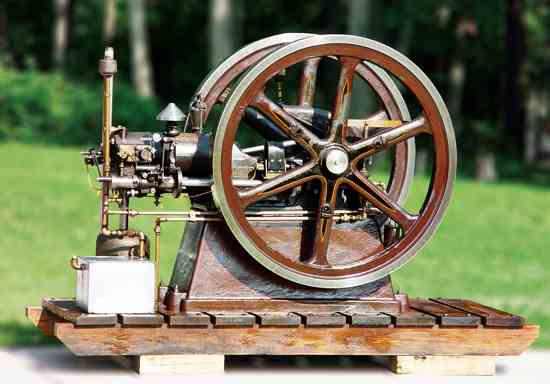
\includegraphics[width=.5\textwidth]{otto_1909.jpg}
  \caption{Motor 1909 5HP Otto Special Electric Lighting de Wayne Grenning}\label{fig:otto1909}
  % https://www.gasenginemagazine.com/gas-engines/1909-5-hp-otto-special-electric/
\end{figure}


Un paso importante hacia los motores actuales fue el desarrollo del ciclo Otto,
propuesto por Nicolaus A. Otto y Eugen Langen, cuyo primer prototipo se puso en
marcha en el año 1876.
%
Otto propuso un motor alternativo con cuatro carreras de pistón: admisión,
compresión, expansión y escape; este prototipo lograba la misma potencia con
mayor eficiencia que los motores de la época con menos de la mitad del peso y
volumen.
%
En la Figura~\ref{fig:otto1909} se ve un motor de ciclo Otto fabricado por
\emph{Otto Gas Engines Works} en el año 1909 en Filadelfia-EEUU.
%
Según la revista \emph{Gas Engine
Magazine}\footnote{\url{https://www.gasenginemagazine.com/gas-engines/1909-5-hp-otto-special-electric/}}
\footnote{ \url{https://www.youtube.com/watch?v=LPSWfg0Y3Hs} } \footnote{
\url{https://www.youtube.com/watch?v=0d0WZ0H56_U} } este motor funcionaba
directamente acoplado a una bomba \emph{TRIPLEX} de agua, como parte de un
sistema de irrigación de un club de campo de Delaware.
%
Los motores han continuado su desarrollo desde entonces, mejorando materiales,
combustibles y procesos de manufactura entre otros aspectos.
%
En las últimas décadas se ha hecho foco en disminuir el consumo de combustible,
nivel de ruido, costo de manufactura, tamaño y las emisiones de gases
contaminantes y de efecto invernadero como las de $CO_2$, $CO$ y $NO_x$, entre
otras.


El ciclo operativo de cuatro tiempos de Otto se puede expresar en términos de
carreras del pistón (véase la Figura~\ref{fig:4tiempos}), en la que se pueden
identificar dos posiciones de interés: el punto muerto superior (PMS) y el punto
muerto inferior (PMI).
%
En el PMS se tiene el volumen mínimo atrapado del cilindro y el pistón está al
final de la carrera, en el punto más alejado del eje del cigüeñal.
%
El PMI es el punto en el que se tiene el volumen máximo del cilindro y el pistón
está en el punto más cercano al eje del cigüeñal, como se ve en la
Figura~\ref{fig:pms_pmi}.
%
Las carreras de pistón del ciclo Otto son:
%
\begin{description}
%
    \item [Carrera de admisión] el pistón se mueve desde el PMS hasta el PMI con
        la válvula de admisión abierta y la de escape cerrada.
        %
        Esto provoca que ingrese una masa de aire o aire-combustible al cilindro.
%
    \item [Carrera de compresión] el pistón se mueve desde el PMI hacia el PMS
        con la válvula de admisión y escape cerradas.
        %
        Esta reducción del volumen comprime y calienta los gases en el interior
del cilindro.
        %
        En una posición angular del ciclo denominada \emph{avance de encendido}
se enciende la mezcla y comienza la combustión.
%
    \item [Carrera de expansión] la combustión produce un gran
aumento de presión y temperatura en el cilindro, la carrera de expansión parte
del PMS hacia el PMI, aprovechando la expansión en volumen de los productos de
la combustión que producen trabajo sobre la cabeza del pistón.
%
    \item [Carrera de escape o barrido] luego de la carrera de expansión, en PMI
se abre la válvula de escape y se produce el  barrido de los gases quemados,
reiniciando el ciclo.
%
\end{description}

\begin{figure}[h!]
  \centering
  \begin{subfigure}{0.6\textwidth}
    \centering
    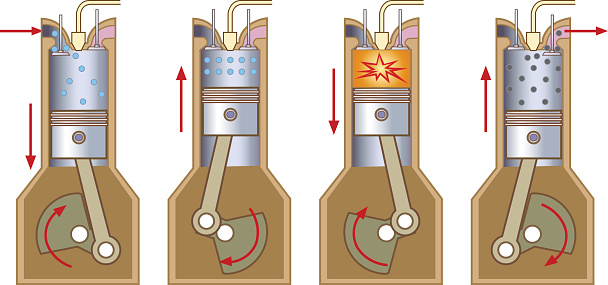
\includegraphics[width=\textwidth]{4stroke.jpg}
    \caption{Ciclo de cuatro tiempos}\label{fig:4tiempos}
  \end{subfigure}%
  \hfill
  \begin{subfigure}{0.4\textwidth}
    \centering
    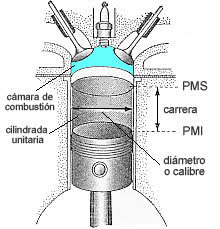
\includegraphics[width=\textwidth]{pms_pmi.jpg}
    \caption{PMS y PMI}\label{fig:pms_pmi}
  \end{subfigure}
  \caption{Ciclo de cuatro tiempos y PMS/PMI}
  \label{fig:4tiempos_pms_pmi} % Etiqueta global para la figura completa
\end{figure}

% https://www.istockphoto.com/es/vector/motor-di%C3%A9sel-de-cuatro-tiempos-gm586705100-100702521

\section{Motores Rotativos}
%
Los motores rotativos son una variante al diseño de los motores alternativos.
%
Su compacidad, balanceo y mayores velocidades de giro los vuelven más atractivos
en aplicaciones en las cuales el volumen es restringido.
%
La mayor velocidad de giro permite alcanzar mayores potencias, por lo que tienen
una menor relación peso/potencia que motores reciprocantes de potencia similar.
%
El diseño rotativo más conocido es el Wankel, cuyo primer prototipo funcional se
desarrolló cerca del año 1957.
%
Existen otros desarrollos de este tipo de motores como el motor rotativo de
pistón líquido, con un ciclo de combustión a volumen constante denominado
HECH~\parencite{hehc_05} y el objeto de este trabajo, el Motor Rotativo de
Combustión a Volumen Constante (MRCVC).

Si bien estos motores son una alternativa interesante a los motores
reciprocantes, la geometría y aspectos constructivos implican que en algunos
casos es necesario introducir aceite mezclado con el lubricante en la cámara de
combustión para lubricar las partes móviles.
%
% Además tienen una mayor superficie de transferencia de calor causando una mayor
% pérdida de calor en comparación con los motores reciprocantes.
%
En la actualidad, los requisitos de niveles de emisiones ambientales de ciertos
gases hacen estos motores inviables para el uso comercial masivo, sin embargo la
compacidad del motor los vuelve atractivos en aplicaciones militares como por
ejemplo para vehículos aéreos no tripulados.

%%%%%%%%%%%%%%%%%%%%%%%%%%%%%%%%%%%%%%%%%%%%%%%%%%%%%%%%%%%%%%%%%%%%%%%%%%%%%%%


\section{Parámetros Operativos e Indicadores de Rendimiento}
%
Para poder comparar entre diferentes diseños de motores se deben conocer algunos
parámetros operativos e indicadores de rendimiento.
%
Algunas de las características más importantes de un motor son:
%
\begin{enumerate}
        %
    \item Potencia y torque
        %
    \item Rango de velocidades de operación
        %
    \item Consumo y costo de combustible
        %
    \item Costo inicial, de operación y de mantenimiento
        %
    \item Confiabilidad
        %
    \item Niveles de ruido y emisiones contaminantes
        %
\end{enumerate}

Estas características se pueden expresar de manera más genérica en función de la
potencia, geometría u otros aspectos de un motor para obtener valores que se
pueden comparar directamente entre motores.
%
Por ejemplo, al cociente entre el trabajo entregado por ciclo y la cilindrada
de un motor se lo conoce como presión media efectiva o \emph{mep}, por sus
siglas en inglés.
%
Algunos parámetros operativos e indicadores se describen en las secciones
siguientes.

%%%%%%%%%%%%%%%%%%%%%%%%%%%%%%%%%%%%%%%%%%%%%%%%%%%%%%%%%%%%%%%%%%%%%%%%%%%%%%%

\subsection{Volumen Desplazado}
%
El volumen desplazado se define como la diferencia entre el volumen máximo
($V_{max}$) y mínimo ($V_{min}$) que ocupa la cámara de combustión:

\begin{equation}\label{eq:vol_desp} V_d = V_{max}-V_{min}
\end{equation}
%
\nomenclature[PO]{\(V\)}{Volumen}
\nomenclature[G]{\(V_d\)}{Volumen desplazado}
% \nomenclature[G]{\(V_{min}\)}{Volumen mínimo en la cámara de combustión}
\nomenclature[G]{\(V_{max}\)}{Volumen máximo de la cámara}

%%%%%%%%%%%%%%%%%%%%%%%%%%%%%%%%%%%%%%%%%%%%%%%%%%%%%%%%%%%%%%%%%%%%%%%%%%%%%%%

\subsection{Relación de Compresión}

Se define como el cociente entre el volumen máximo y el volumen mínimo del ciclo:
%
\begin{equation}\label{eq:rel_comp}
  r_c = \frac{V_{max}}{V_{min}} = \frac{V_d+V_{min}}{V_{min}}
\end{equation}

\nomenclature[G]{\(V_{min}\)}{Volumen mínimo de la cámara}
\nomenclature[PO]{\(r_c\)}{Relación de compresión}
%
Es uno de los parámetros más importantes de un motor ya que afecta a la presión
máxima que se puede obtener en la cámara de combustión, la \emph{performance},
la potencia entregada, los esfuerzos mecánicos y el rendimiento del motor.

%%%%%%%%%%%%%%%%%%%%%%%%%%%%%%%%%%%%%%%%%%%%%%%%%%%%%%%%%%%%%%%%%%%%%%%%%%%%%%%

\subsection{Trabajo Indicado por Ciclo}
%
El trabajo entregado por el gas dentro del cilindro al pistón por cada ciclo de
operación se denomina trabajo indicado por ciclo y se obtiene al integrar la
presión en función del volumen a lo largo de todo el ciclo:

\begin{equation}\label{eq:w_indicado}
  W_{c,i} = \oint p dV
\end{equation}
\nomenclature[PO]{\(W_{c,i}\)}{Trabajo indicado por ciclo}

Para motores de 4 tiempos se debe diferenciar entre trabajo bruto y trabajo neto.
%
En el último se tiene en cuenta el trabajo de bombeo que resulta de la
diferencia del trabajo realizado durante las carreras de admisión y escape, por
lo que este indicador se puede diferenciar en:
%
\begin{description}
  \item [Trabajo indicado bruto por ciclo] $W_{c,ig}$, mide el trabajo realizado
por el motor en las carreras de compresión y expansión.
\nomenclature[PO]{\(W_{c,ig}\)}{Trabajo indicado bruto por ciclo}
        %
  \item [Trabajo indicado neto por ciclo] $W_{c,in}$, mide el trabajo realizado
por el motor considerando las 4 carreras del ciclo.
\nomenclature[PO]{\(W_{c,in}\)}{Trabajo indicado neto por ciclo}
        %
  \item [Trabajo de bombeo] es la diferencia entre el trabajo bruto y neto, y
mide el trabajo realizado durante los procesos de admisión y escape.
  \item [Trabajo de fricción mecánica] es el trabajo consumido por el rozamiento
entre partes móviles del motor.
        %
\end{description}

%%%%%%%%%%%%%%%%%%%%%%%%%%%%%%%%%%%%%%%%%%%%%%%%%%%%%%%%%%%%%%%%%%%%%%%%%%%%%%%

\subsection{Consumo Específico de Combustible y Rendimiento de Conversión del
Combustible}
%
El consumo específico de combustible, \emph{sfc} por sus siglas en inglés, se
define como el cociente entre el caudal másico de combustible ($\dot{m_f}$)
consumido por unidad de potencia $P$ entregada por el motor:
\nomenclature[PO]{\(\dot{m_f}\)}{Caudal másico de combustible}

\begin{equation}\label{eq:sfc} sfc = \frac{\dot{m_f}}{P}
\end{equation}
\nomenclature[PO]{\(sfc\)}{Consumo específico de combustible}

Este parámetro mide la eficiencia con la que el motor utiliza el combustible
para una condición de operación dada.
%
En motores de encendido por chispa se tienen valores típicos de alrededor de
$235\text{g/(kW}\cdot h$~\parencite{heywood}.

Una versión similar de este indicador adimensionalizado en relación a la energía
suministrada por el combustible, es el \emph{rendimiento de conversión del
combustible} $\eta_f$, que se relaciona al \emph{sfc} por medio del poder
calorífico del combustible, $Q_{HV}$.

\nomenclature[PO]{\(Q_{HV}\)}{Poder calorífico}
\nomenclature[PO]{\(\eta_f\)}{Rendimiento de conversión de combustible}

\begin{equation}\label{eq:eta_f} \eta_f = \frac{1}{sfc \cdot Q_{HV}}
\end{equation}

El valor de $Q_{HV}$ es una propiedad del combustible que se determina en un
ensayo de laboratorio.
%
Valores típicos para los combustibles comerciales basados en hidrocarburos son
de 42 a 44 $MJ/kg$.

%%%%%%%%%%%%%%%%%%%%%%%%%%%%%%%%%%%%%%%%%%%%%%%%%%%%%%%%%%%%%%%%%%%%%%%%%%%%%%%

\subsection{Presión Media Efectiva}
%
La presión media efectiva o $mep$ es un indicador cuya variación es proporcional
al torque del motor.
%
El trabajo realizado por ciclo se puede calcular como
$W_c = \frac{P \cdot n_R}{N}$, donde $n_R$ es el número de revoluciones del
cigüeñal por cada ciclo y $N$ son las revoluciones por segundo del eje del motor.
%
Para motores de cuatro tiempos $n_R=2$, y $n_R=1$ para motores de dos tiempos.
%
De este modo, la presión media efectiva se define como:

\begin{equation}\label{eq:mep}
  mep = \frac{W_{c}}{V_d} = \frac{P \cdot n_R}{V_d \cdot N}
\end{equation}
%

Se puede diferenciar entre presión media efectiva indicada (\emph{imep}), al
freno (\emph{bmep}) y de fricción (\emph{fmep}), utilizando el valor de potencia
correspondiente en la ecuación (\ref{eq:mep}).
%
El valor de \emph{mep} (al igual que el torque) de un motor varía con la
velocidad de operación, siguiendo de cerca las tendencias de la curva de
rendimiento volumétrico como se puede ver en el ejemplo de la
Figura~\ref{fig:bmep_tipica}.

En la actualidad, valores típicos de \emph{bmep} de motores de encendido por
chispa (SI por sus siglas en inglés) naturalmente aspirados rondan los 1050 kPa
a 1250 kPa para la velocidad a la que se alcanza el torque máximo~\parencite{heywood}.

\begin{figure}[h!]
  \centering
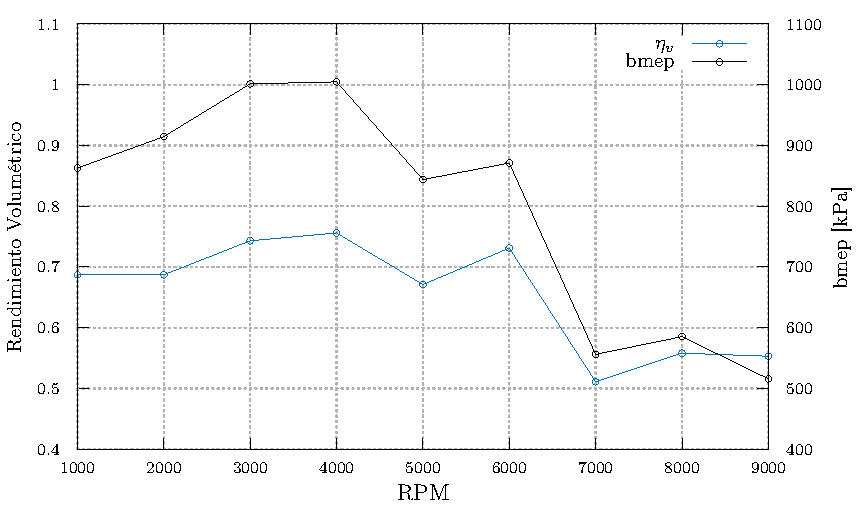
\includegraphics[width=\textwidth]{./gnuplot/bmep_vs_rendVol.pdf}
    \caption{\emph{bmep} y rendimiento volumétrico vs velocidad de operación.}
    \label{fig:bmep_tipica}
\end{figure}

\nomenclature[PO]{\(n_R\)}{Revoluciones de cigüeñal por ciclo}
\nomenclature[PO]{\(N\)}{Velocidad de giro del motor}
\nomenclature[PO]{\(bmep\)}{Presión media efectiva bruta}
\nomenclature[PO]{\(imep\)}{Presión media efectiva indicada}
\nomenclature[PO]{\(mep\)}{Presión media efectiva (\textit{mean effective pressure})}

%%%%%%%%%%%%%%%%%%%%%%%%%%%%%%%%%%%%%%%%%%%%%%%%%%%%%%%%%%%%%%%%%%%%%%%%%%%%%%%

\subsection{Rendimiento Volumétrico}
%
El rendimiento volumétrico mide la eficiencia del sistema de admisión.
%
Es la relación entre el volumen de aire realmente introducido al cilindro y el
volumen teórico que debería entrar al cilindro si este estuviera completamente
lleno con aire a la densidad del ingreso al sistema de admisión ($\rho_{a,i}$).
%
En términos concretos se define como el cociente entre el caudal másico de aire
que ingresa al sistema de admisión ($\dot{m}_{a}$) y la velocidad con la que el
volumen es desplazado por el pistón.
%
En otras palabras, este indicador mide la eficiencia con la que el motor bombea
aire.
\nomenclature[PO]{\(\dot{m}_{a}\)}{Caudal másico de aire}

\begin{equation}\label{eq:eta_v}
  \eta_v = \frac{2\dot{m_a}}{\rho_{a,i}V_d N}
\end{equation}

\nomenclature[PO]{\(\rho_{a,i}\)}{Densidad del aire de admisión}
\nomenclature[PO]{\(m_{a,i}\)}{Masa de aire inductada}

Una forma alternativa a la ecuación anterior es considerando la masa total de aire que
ingresa al cilindro por ciclo, ($m_{a}$):

\begin{equation}\label{eq:eta_v_alt}
  \eta_v = \frac{m_a}{\rho_{a,i}V_d}
\end{equation}

Para motores naturalmente aspirados la densidad del aire de admisión
$\rho_{a,i}$ se toma comúnmente como la densidad atmosférica, por lo que en ese
caso $\eta_v$ mide el rendimiento de todo el sistema de admisión.
%
\nomenclature[PO]{\(\rho_a\)}{Densidad del aire}
\nomenclature[PO]{\(\eta_v\)}{Rendimiento volumétrico}

El valor del rendimiento volumétrico máximo típico para motores naturalmente
aspirados ronda el 90\%~\parencite{heywood}.
%
Su valor se ve afectado por varios fenómenos siendo los más importantes:

\begin{description}
        %
    \item [Efectos cuasiestáticos] Combustible, relación aire/combustible,
vaporización del combustible en el conducto de admisión, temperatura del aire de
admisión, relación entre presión de admisión y escape, relación de compresión,
etc.
  \item [Pérdidas de carga por fricción viscosa] Las pérdidas viscosas aumentan
con la velocidad de flujo y aumentan a medida que aumenta la velocidad de giro
del motor.
        %
Además, se tienen las pérdidas por la presencia de filtros , puertos, válvulas
que generan pérdidas localizadas.
        %
  \item [Transferencia de calor en el sistema de admisión] La mezcla se calienta
por transferencia de calor y esto disminuye la densidad de la misma, reduciendo
la masa de aire.
        %
  \item [Reglaje de las válvulas/puertos] El punto de apertura y cierre de las
válvulas o  puertos (reglaje) es clave para el funcionamiento del motor.
        %
Dependiendo del reglaje que se elija, se puede favorecer el flujo a determinada
velocidad de operación.
        %
    \item [Efecto ram] A grandes velocidades de flujo la inercia del gas al
momento del cierre de la válvula (o puerto) de admisión permite un mayor ingreso
de masa fresca al cilindro.
        %
    \item [Flujo bloqueado en puertos de admisión] En las zonas de
menor área de pasaje la velocidad del fluido puede aumentar hasta alcanzar la
velocidad del sonido, lo cual se conoce como bloqueo y limita el caudal másico que
puede ingresar a la cámara de combustión.
        %
        %
    \item [Sintonía de admisión y escape] El diseño de los sistemas de
admisión y escape puede favorecer el funcionamiento de los mismos a determinada
velocidad de operación, lo cual se logra aprovechando las ondas de presión que
se producen por la apertura y cierre de las válvulas o puertos.
      %
Véanse las secciones~\ref{cap2_sec_sintonia_admision} y~\ref{cap2_sec_sintonia_escape}.
        %
  \item [Sobrecarga] Por medio de un compresor o turbocompresor se puede
aumentar la presión en el sistema de admisión forzando más aire a la cámara de
combustión.
        %
\end{description}

La curva de rendimiento volumétrico es muy similar a la curva de torque o de
presión media efectiva (ver Figura~\ref{fig:bmep_tipica}).
%
La cantidad de aire que ingresa al motor está directamente relacionada con el
trabajo que puede realizar por ciclo de operación.
%
Este indicador es central en la evaluación del desempeño de los sistemas de
intercambio de gases y por este motivo es el principal indicador utilizado en
este trabajo.
%
Se buscó que la curva de rendimiento volumétrico de los motores simulados tenga
un máximo para velocidades cercanas o mayores a 6000 RPM aprovechando el
balanceo mecánico del motor, que permite funcionar y seguir entregando potencia
a altas RPM.
%
La curva debe ser preferentemente suave para todo el régimen de funcionamiento
del motor.
%
Estos y otros efectos se describen en detalle en la
literatura~\parencite{heywood}.
%

Con respecto a la mezcla aire-combustible, se define la relación
de equivalencia $\phi$ a partir del cociente de relaciones combustible/aire (F/A)
de la mezcla y combustible/aire estequiométrica como se indica en la
ecuación~(\ref{eq:phi}).
%
Para más detalles en cuanto a la composición estequiométrica ver la ecuación
~(\ref{eq:estequeometrica}).

\begin{equation}
  \label{eq:phi}
  \phi = \frac{(F/A)_{mezcla}}{(F/A)_{estequiométrica}}
\end{equation}

En estos términos una mezcla pobre en combustible tiene $\phi < 1$, una mezcla
estequiométrica $\phi=1$ y una mezcla rica en combustible $\phi > 1$.


\subsection{Fracción de Gases Residuales}
%
Al final del proceso de barrido, con la válvula de escape cerrada,
pueden quedar gases residuales de la combustión atrapados en el cilindro.
%
Estos gases permanecen para el próximo ciclo de trabajo, afectando el
rendimiento volumétrico, el trabajo obtenido, la eficiencia y las emisiones.
%
La fracción de gases residuales se define como el cociente entre la masa de
gases quemados en el cilindro  al inicio de la fase cerrada del ciclo ($m_{r}$)
y la masa total atrapada en el cilindro ($m$):


\begin{equation}
    x_{r} = \frac{m_{r}}{m}
\end{equation}

\nomenclature[PO]{\(x_{r}\)}{Fracción de gases residuales}
\nomenclature[PO]{\(m_{r}\)}{Masa residual en la cámara de combustión}
\nomenclature[PO]{\(m\)}{Masa total en la cámara de combustión}

En el MRCVC existe un fenómeno llamado solape de cámaras~\parencite{lopez13}.
%
Durante el proceso de admisión de gases frescos, una cámara puede verse afectada
por la apertura del puerto de admisión de la cámara siguiente, que se encuentra
a mayor presión y temperatura debido a que está finalizando el proceso de escape
y comenzando el de admisión, pudiendo provocando un aumento de la cantidad de gases
residuales.


La presencia de gases residuales en la cámara tiene varios efectos en la
combustión y el rendimiento del motor.
%
Algunos pueden ser beneficiosos como la reducción de emisiones nocivas y la
reducción del consumo de combustible.
%
Por otro lado puede tener efectos negativos como la reducción del rendimiento
volumétrico.
%
\begin{description}
        %
  \item[Dilución de la mezcla] el gas residual ocupa volumen que no puede ocupar la mezcla fresca.
        %
  \item[Temperatura] los gases están a mayor temperatura y al mezclarse con la mezcla fresca aumenta su temperatura y volumen, reduciendo la cantidad de mezcla fresca que puede ingresar a la cámara.
        %
  \item[Reducción de $NO_{x}$] un efecto beneficioso es la reducción de emisiones de óxidos de nitrógeno.
        %
  \item[EGR] en motores modernos se recircula gases quemados (\textit{Exhaust Gas Recycle}) para reducir emisiones de $NO_{x}$ y controlar el consumo de combustible. En motores SI se puede utilizar hasta un 30\% de EGR, estos valores son aún mayores para motores de encendido por chispa~\parencite{heywood}.
        %
  \item[Rendimiento volumétrico] la presencia de gases residuales en la cámara disminuye el volumen que puede ocupar la mezcla fresca, lo cual tiene un impacto negativo en el rendimiento volumétrico.
        %
\end{description}

%%%%%%%%%%%%%%%%%%%%%%%%%%%%%%%%%%%%%%%%%%%%%%%%%%%%%%%%%%%%%%%%%%%%%%%%%%%%%%%
\section{Sintonización del Sistema de Admisión}\label{cap2_sec_sintonia_admision}
%
En motores naturalmente aspirados, la apertura de la válvula o puerto de
admisión produce una onda de depresión que viaja desde el puerto de admisión
hacia el extremo opuesto del conducto de admisión.
%
Cuando esta onda de presión llega al pleno de admisión, se refleja como una
onda de sobrepresión que toma un tiempo $t$ en alcanzar nuevamente el puerto.
%
Si el tiempo que toma la onda en reflejarse es tal que alcanza el puerto justo
antes del cierre de la válvula, el sistema está sintonizado.
%
Esta sobrepresión permite que ingrese una mayor cantidad de masa fresca al
cilindro, aumentando la cantidad de trabajo que se puede realizar.

En la Figuras~\ref{fig:sintonia_heywood} se muestran las curvas de presión en
función del ángulo de cigüeñal para un motor operando a $1200$ y $4800$ RPM, en
donde se indican los períodos en los que se encuentran abiertas las válvulas de
admisión (IO) y de escape (EO).
%
Los valores $p_{1}$, $p_{2}$ y $p_{3}$ hacen referencia a diferentes posiciones
a lo largo de los conductos de admisión y escape.
%
Se puede ver que para $p_{1}$ a $4800$ RPM hay un claro pico de presión justo al
cierre del puerto de admisión, el sistema está sintonizado para esta velocidad.

Debido a que la onda de presión debe viajar dos veces la longitud del conducto
de admisión desde el momento que abre el puerto de admisión, para sintonizar el
sistema a bajas velocidades, se requieren longitudes mayores, lo que hace más
grande el sistema de admisión.
%
La sintonía a mayores velocidades de admisión es preferida, porque usualmente se
tiene el máximo de torque y de potencia a mayores RPM, además reduce la
necesidad de conductos más largos.
%
En motores multi-cilíndricos se utiliza un pleno de admisión.
%
Este dispositivo proporciona un volumen grande de aire que sirve el propósito de
cámara de resonancia.
%
Se puede ajustar la resonancia de modo que las oscilaciones de presión internas
produzcan ondas de sobre presión que alcance cada puerto en el momento preciso
en el que se aproxima el cierre del mismo.

\begin{figure}[h!]
  \centering
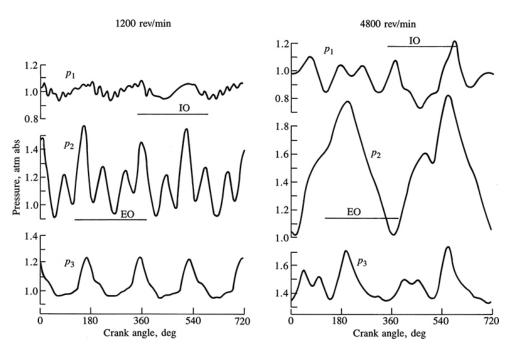
\includegraphics[width=0.8\textwidth]{sintonia_heywood.jpg}
    \caption{Diagrama de presión vs ángulo de cigüeñal~\parencite{heywood}}\label{fig:sintonia_heywood}
\end{figure}

%%%%%%%%%%%%%%%%%%%%%%%%%%%%%%%%%%%%%%%%%%%%%%%%%%%%%%%%%%%%%%%%%%%%%%%%%%%%%%%
\section{Sintonización del Sistema de Escape}\label{cap2_sec_sintonia_escape}

De forma análoga al puerto de admisión, al momento de la apertura del puerto o
válvula de escape los gases residuales de la combustión se encuentran a  mayor
presión que el gas en el conducto.
%
Esto crea una onda de sobrepresión que viaja por el escape hasta alcanzar el
final del mismo o un área de gran volumen, como el catalizador o el silenciador.
%
Desde esta zona se refleja como una onda de depresión, que en caso de alcanzar
el puerto en los instantes previos al cierre del mismo, ayuda a evacuar una
mayor cantidad de gas, disminuyendo la fracción de gases residuales.

En la Figura~\ref{fig:sintonia_heywood} se ve que para el escape en $p_2$ se
tiene una depresión justo al cierre del puerto, este sistema está sintonizado
para 4800 RPM.
%
Es notorio el contraste con el mismo puerto a 1200 RPM, en donde se ve un pico de
presión cerca del cierre del puerto.
%
%%%%%%%%%%%%%%%%%%%%%%%%%%%%%%%%%%%%%%%%%%%%%%%%%%%%%%%%%%%%%%%%%%%%%%%%%%%%%%%

\section{Combustión}
%
La combustión es un proceso en el que se libera la energía química del
combustible.
%
La geometría de un motor de combustión interna permite aprovechar
el aumento de presión y temperatura para convertir energía química en trabajo
mecánico.
%
Los modelos ideales de ciclos operativos se pueden clasificar según el proceso
de combustión en:
%
\begin{enumerate}
        %
    \item Volumen constante, Figura~\ref{fig:comb_vcte}.
        %
    \item Presión constante, Figura~\ref{fig:comb_pcte}.
        %
    \item Presión limitada (parte a volumen constante y parte a presión
constante), Figura.~\ref{fig:comb_plim}.
        %
\end{enumerate}

En un motor de encendido por chispa se tiene una mezcla de aire-combustible en
la cámara de combustión.
%
Dependiendo del tipo de motor, la mezcla se puede formar en el conducto de
admisión, inyectando combustible en algún punto del sistema, se puede producir
la mezcla en la cámara por la inyección directa de combustible.
%
En un motor de encendido por compresión, la mezcla combustible se forma en la
cámara de combustión y la inyección de combustible se realiza directamente en la
cámara, cerca del PMS al final de la carrera de compresión.
%
En este caso las condiciones de presión y temperatura dentro de la cámara producen el
auto-encendido de la mezcla y el inicio del proceso de combustión.

\begin{figure}[h!]
  \centering
  \begin{subfigure}{0.3\textwidth}
    \centering
    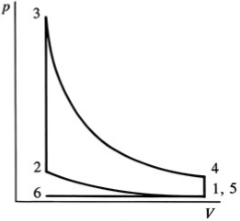
\includegraphics[width=\textwidth]{combustion_vol_cte.png}
    \caption{Volumen Constante}\label{fig:comb_vcte}
  \end{subfigure}%
  \begin{subfigure}{0.3\textwidth}
    \centering
    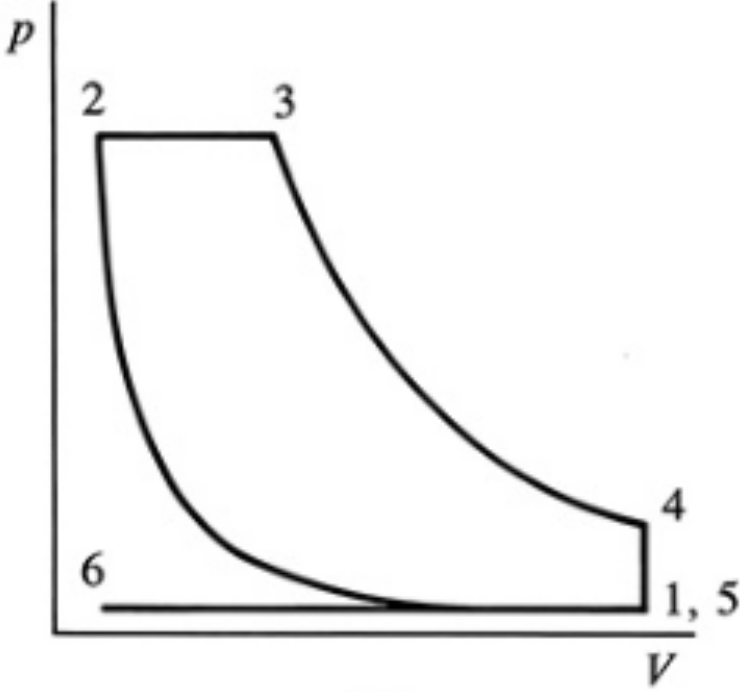
\includegraphics[width=\textwidth]{combustion_presion_cte.png}
    \caption{Presión Constante}\label{fig:comb_pcte}
  \end{subfigure}%
  \begin{subfigure}{0.3\textwidth}
    \centering
    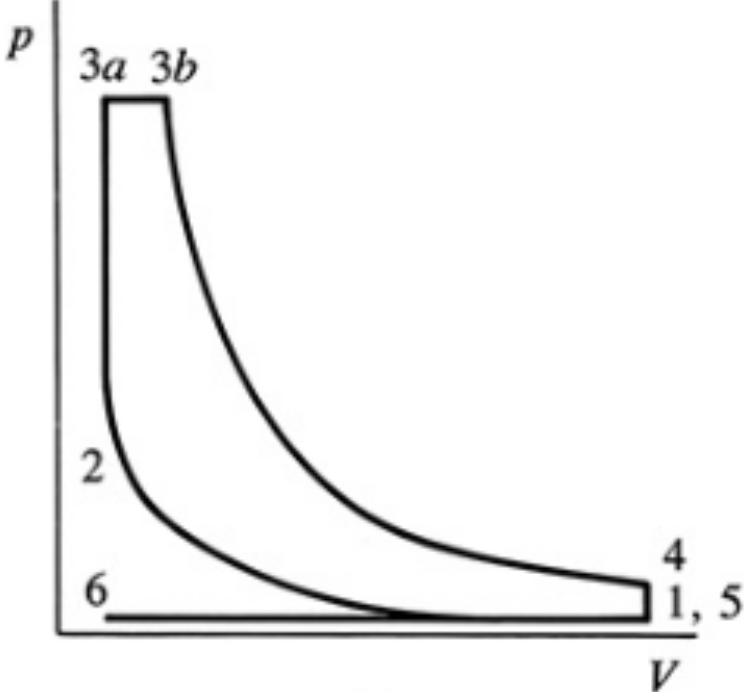
\includegraphics[width=\textwidth]{combustion_presion_limitada.png}
    \caption{Presión Limitada}\label{fig:comb_plim}
  \end{subfigure}
  \caption{Diagramas P-V para ciclos ideales\parencite{heywood}}\label{fig:ciclos_ideales}
\end{figure}

El MRCVC es un motor de combustión interna en el que, debido a su geometría,
gran parte de la combustión ocurre a volumen constante.
%
Esto se puede apreciar en la Figura~\ref{fig:mrcvc_vol_cte}, en la cual se
representa la variación del volumen en función del ángulo del cigüeñal.
%
Para visualizar el mayor rendimiento de la combustión a volumen constante  se
pueden analizar los modelos ideales de ciclos operativos~\parencite{heywood},
considerando un gas ideal con calores específicos constantes como fluido de
trabajo.
%
Se tienen tres casos de combustión: a volumen constante, presión constante o presión
limitada, obteniendo expresiones para el rendimiento de conversión de
combustible~(\ref{eq:rendimiento_p_lim}) y de $imep$ en función de la presión
mínima $p_1$~(\ref{eq:imep_p1}) y máxima $p_3$~(\ref{eq:imep_p3}) del ciclo.
%
Tanto la combustión a volumen constante como a presión constante son casos
extremos de la combustión a presión limitada, por lo que se puede utilizar el
rendimiento de conversión de combustible del ciclo de presión limitada para
comparar entre ambos extremos.

\nomenclature[F]{\(C_{V}\)}{Capacidad calorífica a volumen constante}
\nomenclature[F]{\(C_{P}\)}{Capacidad calorífica a presión constante}

\begin{align}
    \label{eq:rendimiento_p_lim}
    %
  \eta_{f,i} &= 1 - \frac{1}{r_c^{\gamma - 1}} \left[ \frac{\alpha \beta^\gamma-1}{\alpha \gamma (\beta-1)+\alpha-1} \right]\\
  \alpha &= \frac{P_3}{P_2}\\ \beta &= \frac{V_{3b}}{V_{3a}}
    %
\end{align}


\begin{equation}
    \label{eq:Q*} Q^{*}=  \frac{m_{f}Q_{LHV}}{m}
    %
\end{equation}

\nomenclature[PO]{\(Q_{LHV}\)}{Poder calorífico inferior}
\nomenclature[PO]{\(m_{f}\)}{Masa de combustible en la cámara de combustión}


\begin{equation}
    \label{eq:imep_p1} \frac{imep}{p_1} = \frac{Q^*}{c_v T_1 (\gamma-1)} \left( \frac{r_c}{r_c-1} \right) \eta_{f,i}
    %
\end{equation}

\begin{equation}
    \label{eq:imep_p3} \frac{imep}{p_3} = \frac{1}{\alpha r_c^\gamma} \left( \frac{Q^*}{c_v T_1} \right) \left(\frac{1}{\gamma-1} \right) \left( \frac{r_c}{r_c-1} \right) \eta_{f,i}
    %
\end{equation}

En el caso en que  $\alpha=1 \rightarrow P_3=P_2$ se tiene el ciclo de
combustión a presión constante, y en caso de que
$\beta=1 \rightarrow V_{3a}=V_{3b}$ se tiene el ciclo de combustión a volumen
constante (ver Figura~\ref{fig:ciclos_ideales}).

Graficando la ecuación~(\ref{eq:rendimiento_p_lim}) en función de la relación de
compresión $r_c$ (Figura~\ref{fig:rendimientos}), se observa que a igual
relación de compresión, el ciclo a volumen constante presenta mayor rendimiento
de conversión de combustible.

Del mismo modo, graficando la relación entre la presión media efectiva indicada
y la presión máxima del ciclo, $imep/p_3$, se observa que a igual relación de
compresión el ciclo de combustión a presión constante presenta mayores valores
de $imep$ en relación a la presión máxima.
%
Lo cual esta relacionado con las altas presiones alcanzadas en el ciclo ideal de
combustión a volumen constante.
%
La presión máxima que se puede alcanzar en el ciclo real tiene limitaciones
relacionadas a mayores pérdidas de masa (y presión) a través de sellos y la
resistencia mecánica de los componentes del motor.
%
Además, mayores presiones están asociadas con mayores temperaturas en la cámara
de combustión.

\begin{figure}[h!]
  \centering
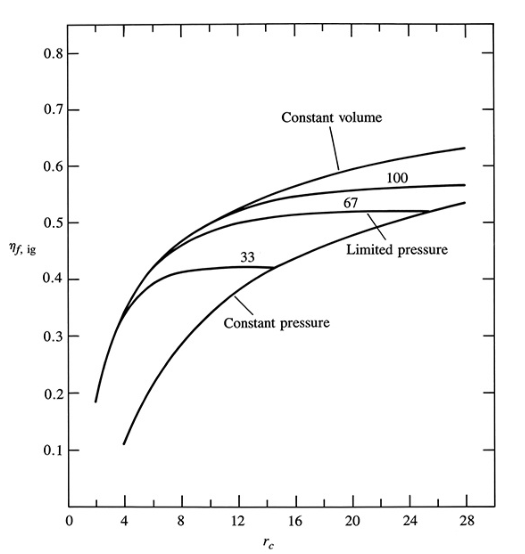
\includegraphics[width=0.6\textwidth]{ciclo/comparativa_rendimientos_ciclos.png}
    \caption{Rendimiento de conversión del combustible en función de $r_c$ para
ciclos de gas ideal de combustión a volumen constante, a presión constante y a
presión limitada~\parencite{heywood}} \label{fig:rendimientos}
    %
\end{figure}


\subsection{Propiedades Termodinámicas de Mezclas aire-combustible}\label{subsec:prop_mezcla}
%
Fue necesario estimar las propiedades termodinámicas de la mezcla para obtener
algunas variables utilizadas para calcular las condiciones iniciales del gas en
las flujometrías.
%
En lo que respecta a la simulación del ciclo del motor, ICESym contiene rutinas
computacionales para calcular el estado termodinámico del fluido de trabajo en
el ciclo operativo.
%
En este apartado se detallan las hipótesis y modelos utilizados en las rutinas
computacionales para el cálculo de las propiedades termodinámicas de las mezclas
de aire-combustible quemadas y sin quemar, para el uso en las condiciones
iniciales requeridas en las flujometrías.

En la simulación del MRCVC se utilizó una mezcla estequiométrica de
aire-isooctano.
%
La reacción estequeométrica para un hidrocarburo genérico se indica en la
ecuación~(\ref{eq:estequeometrica_generica}).

\begin{equation} \label{eq:estequeometrica_generica}
  C_{a}H_{b} + \left(a + \frac{b}{4}\right) \left(O_{2}+3,772N_{2}\right) \rightarrow a CO_{2} + \frac{b}{2} H_{2}O + 3,773 \left(a + \frac{b}{4}\right) N_{2}
\end{equation}

Las rutinas computacionales utilizadas para calcular las propiedades
termodinámicas de las mezclas aire-combustible aproximan las propiedades
químicas de cada especie en la mezcla con curvas polinómicas.

Para cada compuesto $i$ de la mezcla a temperatura estándar $T(K)$ y 1 atmósfera
de presión se aproxima el calor específico a presión constante
$\widetilde{c_{p,i}}$ por la ecuación~(\ref{eq:cp}), la entalpía estándar
$\widetilde{h_{i}}$ por la ecuación~(\ref{eq:h}) y la entropía estándar
$\widetilde{s_{i}}$ por la ecuación~(\ref{eq:s}):

\nomenclature[PO]{\(h_{i}\)}{Entalpía estándar}
\nomenclature[PO]{\(s_{i}\)}{Entropía estándar}

\begin{equation}\label{eq:cp} \frac{\widetilde{c_{p,i}}}{T} = a_{i1} + a_{i2}T + a_{i3}T^{2} + a_{i4}T^{3} + a_{i5}T^{4}
\end{equation}

\begin{equation}\label{eq:h} \frac{\widetilde{h_{i}}}{\widetilde{R}T} = a_{i1} + \frac{a_{i2}}{2}T + \frac{a_{i3}}{3}T^{2} + \frac{a_{i4}}{4}T^{3} + \frac{a_{i5}}{5}T^{4} +\frac{a_{i6}}{T}
\end{equation}

\begin{equation}\label{eq:s} \frac{\widetilde{s_{i}}}{\widetilde{R}} = a_{i1} \ln{T} + a_{i2}T + \frac{a_{i3}}{2}T^{2} + \frac{a_{i4}}{3}T^{3} + \frac{a_{i5}}{4}T^{4} + a_{i7}
\end{equation}

\nomenclature[PO]{\(a_{i}\)}{Coeficiente de polinómicas utilizadas para cálculo de $\widetilde{c_{p}}$, $\widetilde{h}$, $\widetilde{s}$.}

La base de datos seleccionada para el aire y los productos de la combustión es
la utilizada por Chemkin~\parencite{chemkin} y los datos del isooctano fueron
tomados de~\parencite{raine}.

La finalidad de estas rutinas (por fuera de las incluidas en ICESym) es la de
obtener la masa molar de la mezcla $M_{M}$, la viscosidad dinámica $\mu$, el
calor específico a presión constante $C_{P}$, la relación de calores
específicos $\gamma$ y el número de Prandtl $P_{r}$, ya que todos estos valores
son requeridos para obtener las condiciones iniciales de las flujometrías.

La masa molar de la mezcla $M_{M}$ se calcula a partir de la suma de las masas
molares $M_{i}$ y la fracción molar de cada especie química presente en la
mezcla $x_{i}$, ver ecuación~(\ref{eq:mw}).
%
La viscosidad $\mu$ de los productos de la combustión de aire e hidrocarburos
para temperaturas $T\in [500; 4000]K$, presiones $P\in[1; 100]atm$ y relaciones
de equivalencia $\phi \in [0;4]$ se puede aproximar con la
ecuación~(\ref{eq:mu}).
%
Del mismo modo, el número de Prandtl de productos de la combustión de
hidrocarburos y aire se puede estimar en función del $\gamma$ de la mezcla,
para $\phi\leq 1$ con la ecuación~(\ref{eq:pr})~\parencite{heywood}:

\nomenclature[PO]{\(x_{i}\)}{Fracción molar de una especie química ``i''}

\begin{equation}\label{eq:mw}
  M_{M} = \sum_{i} M_{i}x_{i}
\end{equation}

\begin{equation}\label{eq:mu}
  \mu_{productos} = \frac{\mu_{aire}} {1 + 0,027 \phi} = \frac{3,3\times 10^{-7} T^{0,7}} {1 + 0,027 \phi}
\end{equation}

\begin{equation}\label{eq:pr}
    \Pr = 0,05 + 4,2 (\gamma - 1) - 6,7 {(\gamma - 1)}^{2}
\end{equation}

%%%%%%%%%%%%%%%%%%%%%%%%%%%%%%%%%%%%%%%%%%%%%%%%%%%%%%%%%%%%%%%%%%%%%%%%%%%%%%%%%

\section{Coeficiente de Descarga $C_{D}$}\label{sec:cap2_cd}
%
La pérdida de carga localizada en los puertos de admisión y escape se puede
representar a través del coeficiente de descarga, $C_{D}$.
%
Este coeficiente varía con la geometría y condiciones de operación del puerto,
siendo $C_{D}=1$ el caso ideal sin pérdida de carga localizada.
%
Es un parámetro importante porque permite obtener una mejor estimación del flujo
másico real en el puerto y se define como:

\begin{equation}
  C_{D} = \frac{\text{flujo másico real}}{\text{flujo másico ideal}}
\end{equation}

El $C_{D}$ de un puerto se puede obtener experimentalmente en un banco de prueba
mediante un ensayo que consiste en medir el caudal que circula por un puerto con
una presión de descarga fija que, en equipos comerciales varía entre $250-700$
mm.c.a.
%
Comúnmente estos ensayos se realizan en un banco que incluye solamente la tapa
de cilindros y una camisa que simula el cilindro de la cámara de combustión,
dejando de lado otros elementos del sistema como pistón, los conductos de
admisión y otros.
%
En la imagen~\ref{fig:banco_flujometrias} se muestra un banco de pruebas
comercial.

\begin{figure}[h!]
  \centering
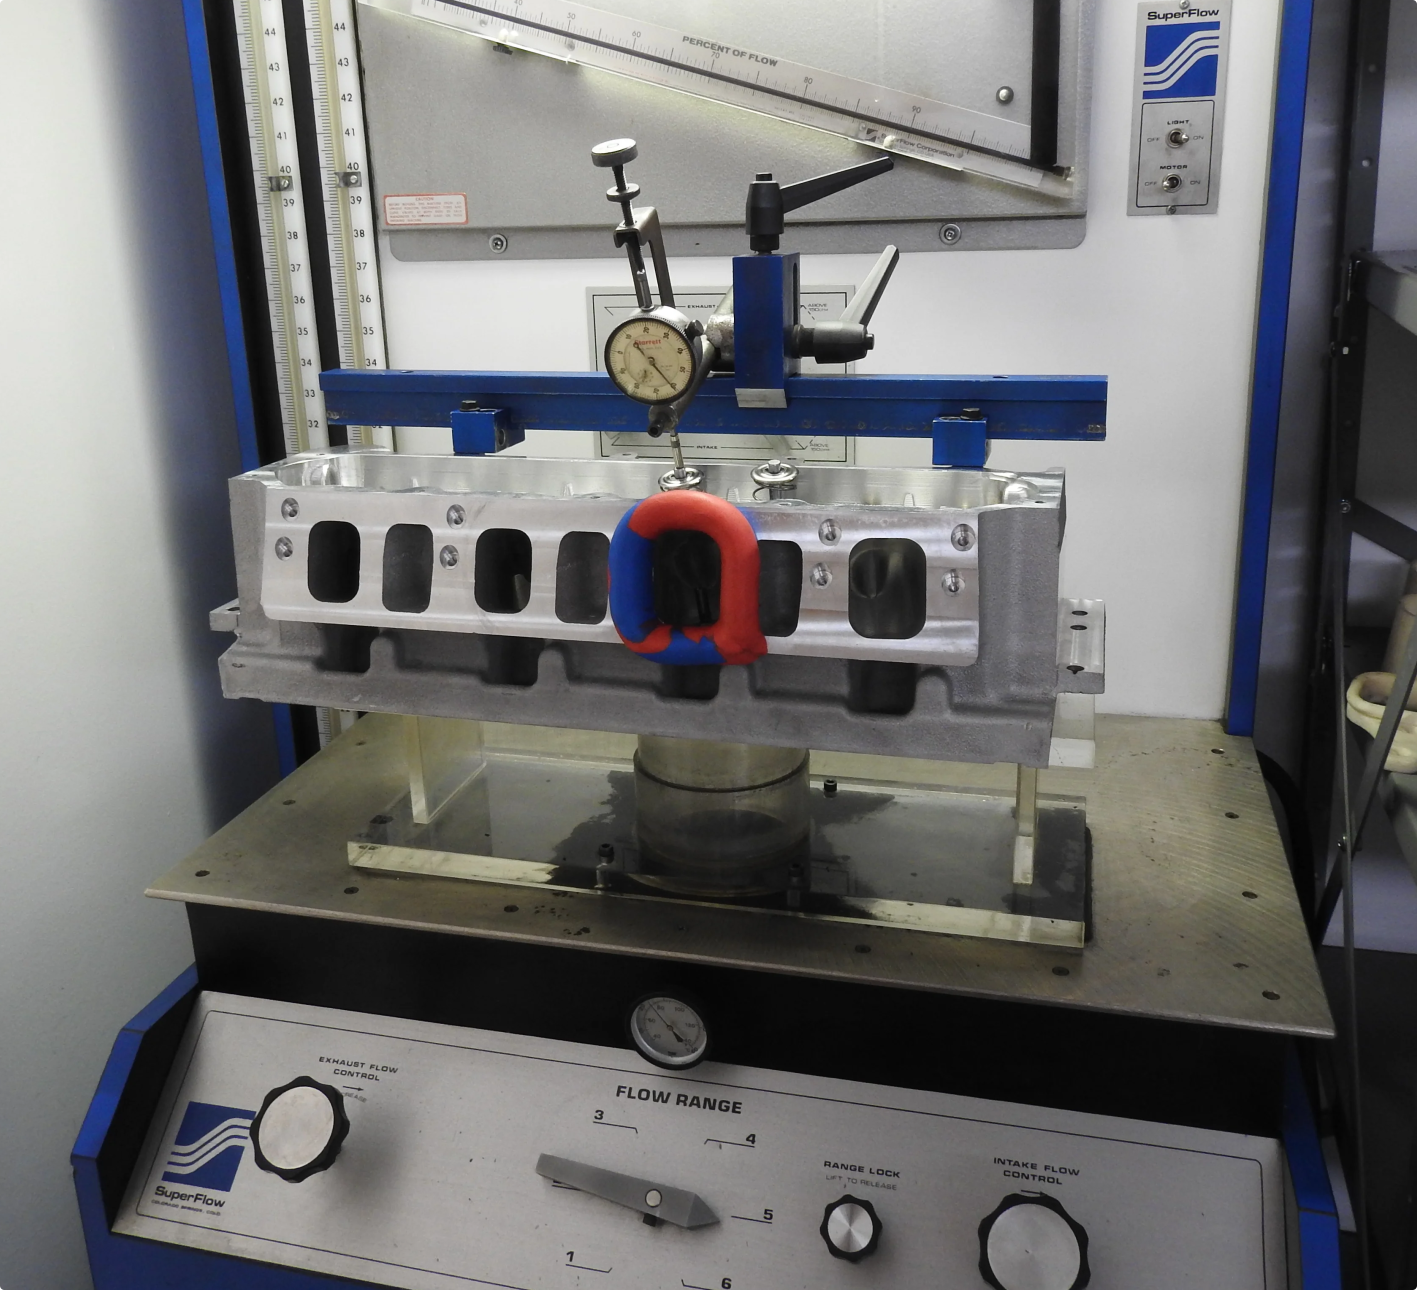
\includegraphics[width=0.5\textwidth]{./flujometrias/banco_flujometrias.png}
  \caption{Banco de flujometrías Super-Flow SF-750}\label{fig:banco_flujometrias}
\end{figure}

Durante el ensayo se mide el caudal de aire atmosférico para diferentes grados
de apertura de la válvula y así se obtienen datos de (alzada, flujo) con los
cuales comparar entre diferentes geometrías de puertos de admisión o escape.
%
En la Figura~\ref{fig:flow-1} se muestra el resultado del ensayo de un
flujómetro en el que se compara la capacidad de flujo de dos tapas de cilindro
diferentes de un BMW S14
\footnote{\url{http://e30sport.net/tech_articles/engine-tech/flow-1/chart-1.htm}}.

\begin{figure}[h!]
  \centering
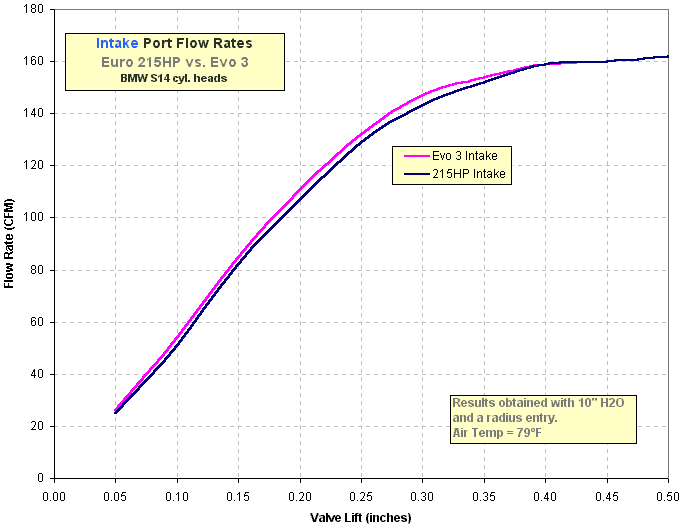
\includegraphics[width=0.8\textwidth]{./flujometrias/flow-1.png}
  \caption{Comparación entre flujometrías de dos tapas de cilindro de un BMW S14}\label{fig:flow-1}
\end{figure}

Otra forma de aproximar un coeficiente de descarga es por medio de flujometrías
computacionales.
%
El uso de CFD permite modelar el puerto en condiciones operativas, incluyendo
la interacción con elementos como por ejemplo el pistón, o en el caso del
MRCVC, estator y conjunto rotante.
%
Además, se pueden modelar las propiedades del fluido de trabajo para una
viscosidad, presión y temperatura representativas de las condiciones operativas
del motor que se está simulando.
%
En este trabajo se optó por esta metodología, es decir, a partir de las flujometrías se
obtuvo un valor de caudal másico el cual es utilizado para calcular un
coeficiente de descarga.

Conociendo el caudal másico $\dot{m}$, el valor de $C_{D}$  se calcula con las
ecuaciones de flujo compresible a través de una restricción, habiendo dos casos
distintivos: flujo bloqueado y no bloqueado.

Para el caso en que el flujo no esté bloqueado la ecuación de $\dot{m}$ es
la~(\ref{eq:m_no_bloqueado}) y en caso de que se cumpla la
desigualdad~(\ref{eq:cond_bloqueo}) el flujo está bloqueado y se utiliza la
ecuación~(\ref{eq:m_bloqueado}):
%

\begin{equation}\label{eq:m_no_bloqueado}
    \dot{m} = \frac{C_D A_R p_0}{\sqrt{R T_0}} {\left(\frac{p_T}{p_0} \right)}^{1/\gamma} {\left( \frac{2\gamma}{\gamma-1} \left[1- {(\frac{p_T}{p_0})}^{{(\gamma-1)}/\gamma} \right] \right)}^{1/2}
\end{equation}

\begin{equation}\label{eq:cond_bloqueo}
  \frac{p_T}{p_0} \le {[\frac{2}{\gamma+1}]}^{\gamma/(\gamma - 1)}
\end{equation}

\begin{equation}\label{eq:m_bloqueado}
  \dot{m}=  \frac {C_D A_R p_0} {{(R T_0)}^{1/2}} \gamma^{1/2} {\left( \frac{2}{\gamma+1} \right)}^{(\gamma+1)/(2(\gamma-1))}
\end{equation}

donde
\begin{itemize}
    \item $p_0$, es la presión de estancamiento antes de la restricción.
    \item $T_0$, es la temperatura de estancamiento antes de la restricción.
    \item $p_T$, es la presión estática justo después de la restricción.
    \item $A_R$, es el área de pasaje de flujo o de referencia.
    \item $\dot{m}$, es el caudal másico.
  \item $\gamma$, es el cociente de capacidades térmicas del gas.
\end{itemize}

\nomenclature[PO]{\(p_0\)}{Presión de estancamiento antes de la restricción}
\nomenclature[PO]{\(T_0\)}{Temperatura de estancamiento antes de la restricción}
\nomenclature[PO]{\(p_T\)}{Presión estática justo después de la restricción}
\nomenclature[G]{\(A_R\)}{Área de pasaje de flujo o de referencia}

El flujo está bloqueado si la velocidad en la garganta de la restricción
alcanza la velocidad sónica. 
%
Dada esta condición $\dot{m}$ alcanza un límite y reducir la presión aguas
abajo de la restricción no produce un aumento del caudal.
%
% La condición de flujo bloqueado se puede expresar en términos de la relación
% de presiones aguas arriba $p_{0}$ y aguas abajo de la restricción $p_{T}$.
%
Las presiones y temperaturas involucradas en el cálculo de $\dot{m}$ se pueden
medir u obtener de una simulación computacional del ciclo del motor.
%
\nomenclature[PO]{\(p,P\)}{Presión}

Un parámetro importante en las ecuaciones utilizadas para el cálculo del
coeficiente de descarga $C_{D}$ es el área de referencia $A_{R}$ que define el
área utilizada para calcular el caudal másico que circula por el puerto.
%
% En un motor con válvulas se suele tomar el área de cortina como el producto de
% la circunferencia de la válvula con la alzada, es decir:

La elección del área de referencia utilizada para el cálculo es arbitraria.
%
Sin embargo en un motor con válvulas se suele utilizar el área de cortina (ver
Figura~\ref{fig:area_cortina}) la cual es el producto del perímetro de la
cabeza y la alzada de válvula.

\begin{equation} \label{eq:area_cortina}
  A_R = A_C = \pi D_v l_v
\end{equation}

% \nomenclature[G]{\(A_R\)}{Área de pasaje de flujo o de referencia}
\nomenclature[G]{\(A_C\)}{Área de cortina}
\nomenclature[G]{\(D_v\)}{Diámetro de válvula}
\nomenclature[G]{\(l_v\)}{Alzada de válvula}

\begin{figure}[h!]
  \centering
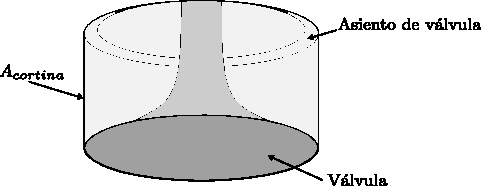
\includegraphics[width=0.5\textwidth]{valve_curtain.pdf}
  \caption{Área de cortina}\label{fig:area_cortina}
\end{figure}

Los valores de densidad, velocidad, presión y temperatura se obtienen de los
datos de salida de ICESym para un puerto, ángulo y velocidad dada.
%
Para la temperatura se utiliza la temperatura de la cámara, $T_0 = T_C$, la
presión antes y después del puerto se selecciona de acuerdo al sentido de
flujo.
%
En caso de ser hacia la cámara de combustión la presión en el puerto se utiliza
como inicial $P_0$ y la presión en la cámara es la aproximación a la presión en
la restricción $P_T$.
%
\nomenclature[PO]{\(T\)}{Temperatura}
%
\nomenclature[SU]{\(0\)}{Valor inicial}

El valor de $\gamma$ se obtiene de las propiedades de la mezcla con las rutinas
computacionales descritas en el apartado~\ref{subsec:prop_mezcla}.
